\section{Appendix}

Figure~\ref{fig:switch_resources} provides a breakdown of the resource
consumption of Swordboxes components. We collected these values from our
experimental setup on an Edge Core Wedge 100BF-65X using the barefoot SDE
version 9.7.0. Each reported percentage is the average value across the total 16
switch pipeline stages. {\sword} fits into 8 stages, and is run entirely on the
ingress pipeline.

\textbf{Switch Resource Utilization}
\begin{figure}[t]
    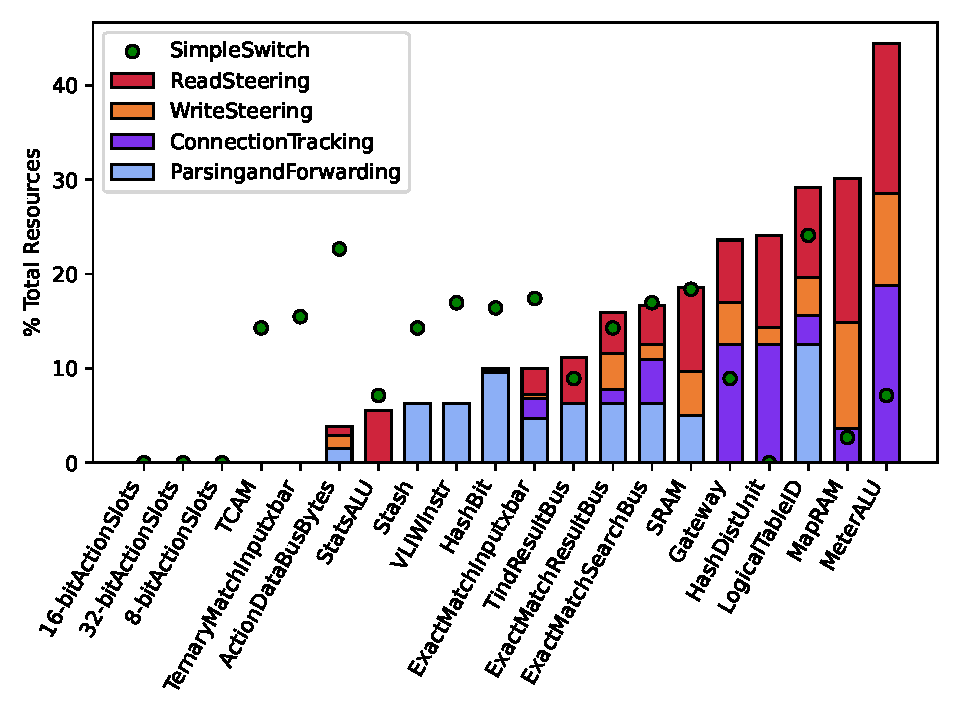
\includegraphics[width=0.485\textwidth]{fig/switch_resources.pdf}
%  \vskip -0.5em
    \caption{Breakdown of switch resource utilization by swordbox component}
    \label{fig:switch_resources}
%      \vskip -0.5em
\end{figure}

\subsection{Packet Size}

{\sword} is designed to run at line rate, and is unperturbed by packet size. In
the case of Clover, it's retries require a significant bandwidth overhead which
causes additional slowdown when payloads are large.
Figure~\ref{fig:packet_size}, shows how {\sword} reacts to changes in packet
sizes. At 128 bytes the limitation is the load applied by clients. At 256 bytes
and above the 100gbps limit of the ConnectX-5 NICs becomes the bottleneck for
read and write steering, and the throughput drops proportionally. In the case of
Clover retries on larger packets are more expensive than on smaller packets
because the retry consumes additional bandwidth on an already saturated link.

\begin{figure}
  \centering
  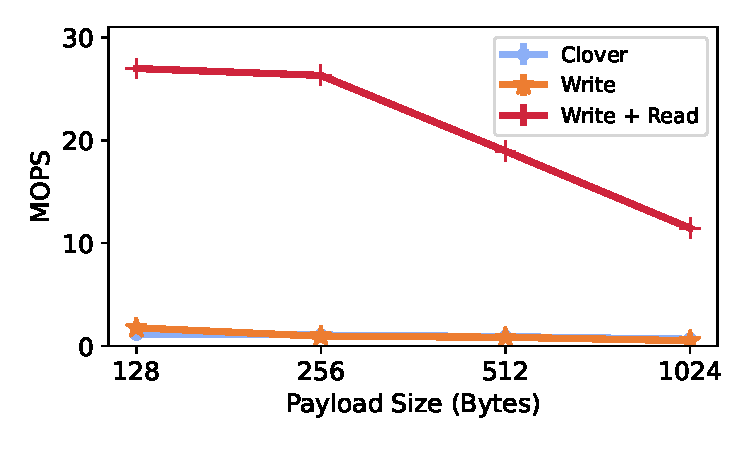
\includegraphics[width=0.485\textwidth]{fig/packet_size.pdf}

    \caption{Performance across RDMA payload sizes using 400 client cores at a
    50 percent read 50 percent write ratio.}

    \label{fig:packet_size}
\end{figure}

\subsection{Contention}

{\sword} is designed to operate well under even extreme contention. We test it's
ability by generating workloads at different points across a zipf distribution.
The community standard for zipf is 0.99, at this ratio the most frequently
requested key is requested around 17\% of the time. We measure further down the
distribution up to zipf of 1.5, at which point the hottest key is requested over
50\% of the time, and the second hottest is around 20\%.
Figure~\ref{fig:contention} shows that in the face of high contention 1.0 and
above write and read steering yields a 40x and above performance improvement at
a 50\% write workload. The decrease in read and write performance at high
contention is due to Clover's block allocator which becomes a bottleneck when
keys are requests more than 30\% of the time.

\begin{figure}
  \centering
  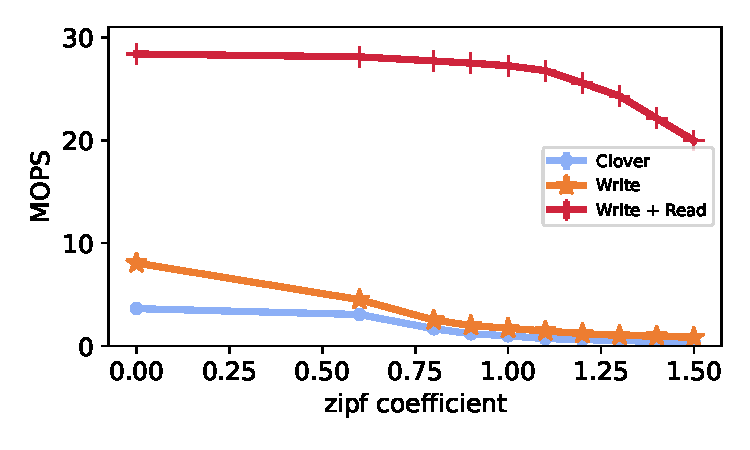
\includegraphics[width=0.485\textwidth]{fig/contention.pdf}

    \caption{Performance as contention increases with zipf coefficient using 400
    client cores on a 50\% write workload}

    \label{fig:contention}
\end{figure}
